\documentclass[12pt, a4paper]{report}
\usepackage{epsfig}
\usepackage{subfigure}
%\usepackage{amscd}
\usepackage{amssymb}
\usepackage{graphicx}
%\usepackage{amscd}

\usepackage{subfiles}
\usepackage{framed}
\usepackage{subfiles}
\usepackage{amsthm, amsmath}
\usepackage{amsbsy}
\usepackage{framed}
\usepackage[usenames]{color}
\usepackage{listings}
\lstset{% general command to set parameter(s)
basicstyle=\small, % print whole listing small
keywordstyle=\color{red}\itshape,
% underlined bold black keywords
commentstyle=\color{blue}, % white comments
stringstyle=\ttfamily, % typewriter type for strings
showstringspaces=false,
numbers=left, numberstyle=\tiny, stepnumber=1, numbersep=5pt, %
frame=shadowbox,
rulesepcolor=\color{black},
columns=fullflexible
} %
%\usepackage[dvips]{graphicx}
\usepackage{natbib}
\bibliographystyle{chicago}
\usepackage{vmargin}
% left top textwidth textheight headheight
% headsep footheight footskip
\setmargins{3.0cm}{2.5cm}{15.5 cm}{22cm}{0.5cm}{0cm}{1cm}{1cm}
\renewcommand{\baselinestretch}{1.5}
\pagenumbering{arabic}
%\theoremstyle{plain}
\newtheorem{theorem}{Theorem}[section]
\newtheorem{corollary}[theorem]{Corollary}
\newtheorem{ill}[theorem]{Example}
\newtheorem{lemma}[theorem]{Lemma}
\newtheorem{proposition}[theorem]{Proposition}
\newtheorem{conjecture}[theorem]{Conjecture}
\newtheorem{axiom}{Axiom}
\theoremstyle{definition}
\newtheorem{definition}{Definition}[section]
\newtheorem{notation}{Notation}
\theoremstyle{remark}
\newtheorem{remark}{Remark}[section]
\newtheorem{example}{Example}[section]
\renewcommand{\thenotation}{}
%\renewcommand{\thetable}{\thesection.\arabic{table}}
%\renewcommand{\thefigure}{\thesection.\arabic{figure}}

\author{ } \date{ }

\begin{document}
\author{Kevin O'Brien}
\title{Mixed Models for Method Comparison Studies}
\tableofcontents



\newpage
\chapter{Model Diagnostics for Method Comparison}
Linear Mixed Effects models are a useful framework for fitting a wide range of models. However, they are known to be sensitive to outliers, specifically the likelihood based estimation techniques, such as ML and REML. 

A full and comprehensive analysis that comprises residual analysis and influence analysis for testing model assumptions, should be carried out. Therefore, a suite of diagnostic procedures should be specified for method comparison in mind. However it has been noted by several papers \citep{Christensen, schabenberger} that model diagnostics do not often accompany LME model analyses. 

Further to the analysis of residuals, \citet{schabenberger} recommends the examination of the following questions:
\begin{itemize}
	\item Does the model-data agreement support the model assumptions?
	\item Should model components be refined, and if so, which components? 
	%%- For example, should certain explanatory variables
	%%- be added or removed, and is the covariance of the observations properly specified?
	\item Are individual data points or groups of cases particularly
	influential on the analysis?
\end{itemize}
The last of these three questions, regarding influential points, is of particular interest in the context of method comparison. After fitting an LME model, it is important to carry put model diagnostics to check whether distributional assumptions for the residuals as satisfied and whether the fit the model is sensitive to unusual assumptions. 

%Model validation and model appraisal are vital parts of the modelling process, yet are too often overlooked. Using a small set of simple measures and methods, such as the AIC and $R^2$ measures, is insufficient to properly assess the usefulness of a fitted model.

Model diagnostics techniques determine whether or not the distributional assumptions are satisfied, and to assess the influence of unusual observations. For classical linear models model diagnostics are now considered a required part of any statistical analysis, and are commonly available in statistical packages and standard textbooks on applied regression.


Model diagnostic techniques, well established for classical models, have since been adapted for use with linear mixed effects models. \citet{schabenberger} remarks that the concept of critiquing the model-data agreement applies in LME models in the same way as in classical linear models. \citet{west} argues that model and data diagnostics are even more important because of the more complex model structure. 


Diagnostic techniques for LME models are inevitably more difficult to implement, due to the increased complexity. \citet{Christensen} advises that outlier identification is necessary before any conclusions may be drawn from the fitted model, with the leverage of an observation a further consideration. \citet{schabenberger} discusses the state of LME diagnostics tools, providing a useful summary of established measures. Prominent in literature is the taxonomy of residuals for LME Models, distinguishing between condition residuals, marginal residuals and EBLUPS, including \citet{hilden1995, schabenberger, west, NobreSinger2007}. 


\section{Residual Analysis}
Analysis of residuals, the differences between observed values and fitted values, is a widely used model validation technique used to examine model assumptions, as well as to detect outliers and potentially influential data points. 

As with classical models, there are two key graphical techniques: a residual plot and the normal probability plot. The rationale is that, if the model is properly fitted to the model, then the residuals would approximate the random errors that one should expect. If the residuals behave randomly, with no discernible trend, the model has fitted the data reasonably well. 
%If some sort of non-random trend is evident in the model, then the model can be considered to be poorly fitted. 

The underlying assumptions for LME models are similar to those of classical linear models. However, for LME models the matter of residuals are more complex, both from a theoretical point of view and from the practicalities of implementing a comprehensive analysis using statistical software.

Statistical software environments, such as the \texttt{R} programming language, provides a suite of tests and graphical procedures for appraising a fitted LME model, with several of these procedures analysing the model residuals. Texts such as \citet{PB,west,Galecki} describe what can be implemented for LME residual analyses with statistical software, such as \texttt{R} and \texttt{SAS}.


%The figures on the next page depict the residual analysis for the \textit{Blood} data, which can be used to indicate which methods disagree with the rest, but these would be a confirmation of something detected previously.

%-- \subsection*{Residual Plots}
Residual diagnostics are typically implemented as a plot of the observed residuals and the predicted values. A visual inspection for the presence of trends inform the analyst on the validity of distributional assumptions, and to detect outliers and influential observations.



Analysis of the residuals could determine if the methods of measurement disagree systematically, or whether or not erroneous measurements associated with a subset of the cases are the cause of disagreement. 

In the context of method comparison, a residual analysis would be carried out just as any other LME model would, testing normality. \citet{PB} provide some insight into how to compute and interpret model diagnostic plots for LME models. Unfortunately this aspect of LME theory is not as expansive as the corresponding body of work for linear models.
 
 Residual analysis must be carried out on a method-by-method basis, for a model fitted by Roy's approach. When considering the whole data, erroneous conclusions will be drawn.

Figure \ref{fig:ResidPlot} depicts residual plots for Roy's model for the systolic blood pressure data used in \citet{BA99}. Inspection of the normality probability plot would lead to the conclusion that the key assumption of residual normality being invalid. However, this plots depicts two difference populations of residuals, an incorrect use of the normal probability plot, and therefore it is not possible to tell if the assumption of normality for residuals is invalid.

\begin{figure}[h!]
	\centering
	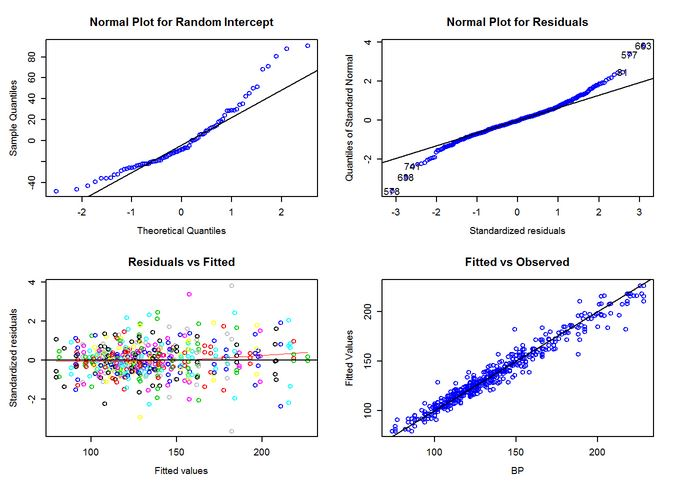
\includegraphics[width=0.9\linewidth]{images/ResidPlot}
	\caption{}
	\label{fig:ResidPlot}
\end{figure}


% Points are labelled by subjects, with cases 67, 68 and 71 being among the prominent cases. 
% Prominent cases warrant further investigation, but an analyst should procede to influence diagnostics beforehand.

% As the LME model can be tailored to the needs of the particular research question, the rationale behind the model appraisal must 
% follow accordingly. 

For method comparison studies, one should create plots specific to each method, useful in determining which methods disagree with the rest.

Figure~\ref{bloodnlme-ResidPlot} depicts residual plot for the Systolic Blood Pressure example, panelled by the various measurement methods, confirming agreement between methods J and R. Lack of agreement between those two methods and method S is also indicated. However, little insight can be gained as to what actually causes this lack of agreement. 
\begin{figure}[h!]
	\centering
	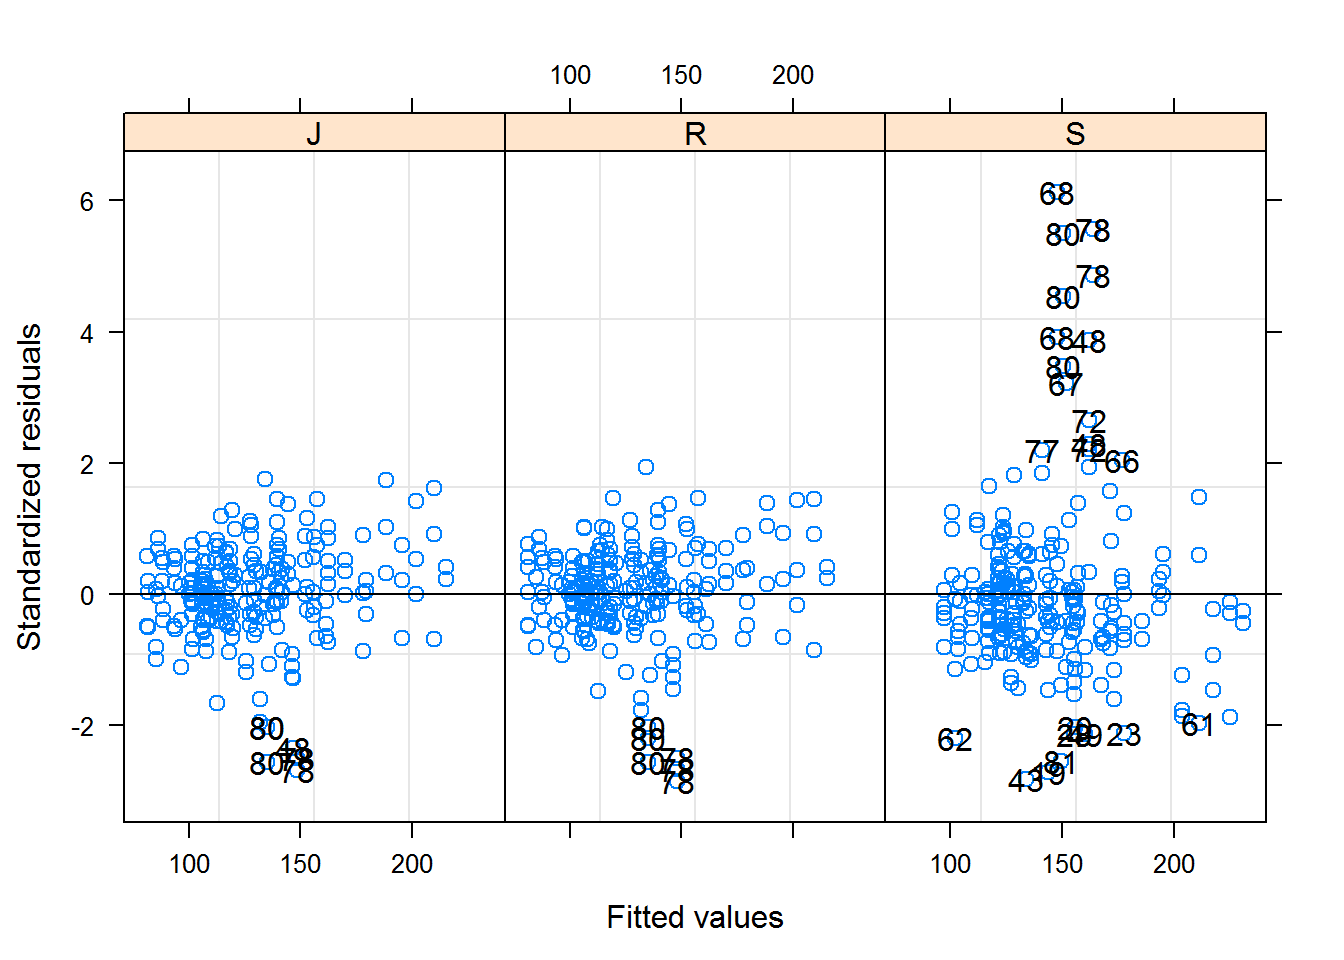
\includegraphics[width=0.8\linewidth]{images/bloodnlme-ResidPlot}
	\caption{LME Residuals by Method (Blood Pressure Data)}
	\label{bloodnlme-ResidPlot}
\end{figure}



%\begin{figure}[h!]
%\centering
%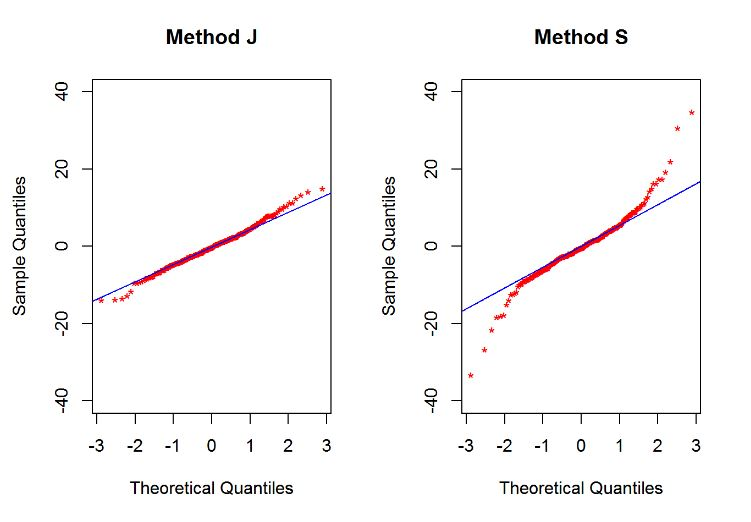
\includegraphics[width=1.1\linewidth]{images/Resid-newplot2}
%\caption{}
%\label{fig:Resid-newplot2}
%\end{figure}


%The fitted model used in the Blood data example, \texttt{JS.ARoy20091}, was fitted using the \texttt{lme()} function from the nlme package, and as such, is stored as an \texttt{lme} object. The \texttt{residual} functions extracts residuals of a fitted LME model, depending on the type of residual required.
%


% \subsubsection{LME Residuals}
% LME are flexible tools for the analysis of clustered and repeated measurement data. LME extend the capabilities of standard linear models by % allowing unbalanced and missing data, as long as the missing data are MAR. Structured covariance matrices for both the random effects G and % the residuals R. 



\subsubsection{Taxonomy of LME Residuals}
Standard residual and influence diagnostics for linear models can
be extended to linear mixed models. The dependence of
fixed-effects solutions on the covariance parameter estimates has
important ramifications in perturbation analysis. To properly assess the
full impact of a set of observations on the analysis, covariance
parameters need to be updated, which requires refitting of the
model.
%---http://www.stat.purdue.edu/~bacraig/notes598S/SUGI_Paper_Schabenberger.pdf

\citet{PB} describes three types of residual that describe the variabilities
present in LME models, marginal residuals which predict marginal errors, conditional residual, which predict conditional errors, and the BLUP, $ {Z\hat{b}}$, that predicts random effects. Each type of residual is useful to evaluates some assumption of the model.

The conditional (subject-specific) and marginal (population-averaged) formulations in the linear mixed model enable you to consider conditional residuals that use the estimated BLUPs of the random effects, and marginal residuals which are deviations from the overall mean. The definitions of both marginal residuals ($r_m$) and conditional residuals ($r_c$) follow from the definitions of marginal and conditional means in the LME model 
$E[{Y}] = {X}{\beta}$ and $E[{Y|{u}}] = {X}{\beta} + {Z}{u}$, respectively.

A marginal residual is the difference between the observed data and the estimated marginal mean, i.e. $r_{Mar} = y - X \hat{\beta}$. A conditional residual is the difference between the observed data and the predicted value of the observation. 
 Conditional residuals include contributions from both fixed and random effects, whereas marginal residuals include contribution from only fixed effects. Marginal residuals should have mean of zero, but may show grouping structure. Also they may not be homoscedastic. In a model without random effects, both sets of residuals coincide.



Residuals using the BLUPs are useful to diagnose whether the random effects components in the model are specified correctly, marginal residuals are useful to diagnose the fixed-effects components.

%- http://www.ime.usp.br/~jmsinger/MAE5705/EMR2013.pdf

According to \citet{hilden1995}, a residual is considered pure for a specfic type of error if it depends only on the fixed components and on the error that it is supposed to predict. Residuals that depend on other types of error are known as `confounded errors'.





%In linear mixed effects models, diagnostic techniques may consider `conditional' residuals. A conditional residual is the difference between an observed value $y_{i}$ and the conditional predicted value $\hat{y}_{i} $.
%
%\[ \hat{epsilon}_{i} = y_{i} - \hat{y}_{i} = y_{i} - ( X_{i}\hat{beta} + Z_{i}\hat{b}_{i}) \]
%



%==========================================================================%
\section{Influence Diagnostics}
Model diagnostic techniques can determine whether or not the distributional assumptions are satisfied, but also to assess the influence of unusual observations. Following model specification and estimation, it is of interest to explore the model-data agreement by raising pertinent questions. 

\citet{west} remarks that influence diagnostics play an important role in the interpretation of results, because influential data can negatively influence the statistical model and generalizability of the model. 
 

Unfortunately this aspect of LME theory is not as expansive as the corresponding body of work for classical linear models. \citet{PB} provide some insight into how to compute and interpret model diagnostic plots for LME models. Their particular observations will be reverted to shortly. 


Influence diagnostics are formal techniques that allow the identification observation that heavily influence estimates of the estimates of fixed effects and variance covariance parameters.


Influential points are a set of one or more observations whose removal would cause a different conclusion in the analysis, e.g. substantially affect estimates. 
Influential points have a large influence on the fit of the model. Influential points are a set of one or more observations whose removal would cause a different conclusion in the analysis, e.g. substantially changes the estimate of the regression coefficients. 




The process of carrying out model diagnostic involves several informal and formal techniques, which will mentioned throughout the chapter.




One approach for determining influential points is to compare the fit of the model with and without each observation. The basic rationale behind identifying influential data is that when iteratively single units are omitted from the data, models based on these data should not produce substantially different estimates. 


\subsection*{Procedure for Quantifying Influence}






\citet{schabenberger} describes a simple procedure for quantifying influence for LME Models. Firstly a model should be fitted to the data, and estimates of the parameters should be obtained. 

The second step is that either single or multiple data points, specifically outliers, should be omitted from the analysis, with the original parameter estimates being updated. This is known as \textit{``leave one out"} or \textit{``leave k out"} analysis. 

The final step of the procedure is comparing the sets of estimates computed from the entire and reduced data sets to determine whether the absence of observations changed the analysis. 


%http://support.sas.com/documentation/cdl/en/statug/63033/HTML/default/viewer.htm#statug_mixed_sect024.htm

%http://www.itl.nist.gov/div898/handbook/pmd/section4/pmd44.htm
\subsection{Comparing Influence and Residual Analysis}
%In LME models, there are two types of residuals, marginal residuals and conditional residuals. A
%marginal residual is the difference between the observed data and the estimated marginal mean. A conditional residual is the
%difference between the observed data and the predicted value of the observation. In a model without random effects, both sets of residuals coincide \citep{schab}.

\citet{influenceLME4} compares residual analysis and influence analysis. Cases with high residuals (defined as the difference between the observed and the predicted scores on the dependent
variable) or with high standardized residuals (defined as the residual divided by the standard deviation
of the residuals) are indicated as outliers.

However, an influential case is not necessarily an outlying residual. On the contrary: a strongly influential case dominates
the regression model in such a way, that the estimated regression line lies closely to this case. The analysis of residuals cannot be used for the detection of influential cases \citep{crawley2012r}.







\subsection*{Case Deletion}

The impact of an observation on a regression fitting can be determined by the difference between the estimated regression coefficient of a model with all observations and the estimated coefficient when the particular observation is deleted. 

The subscript $(U)$ is used to denote quantities computed from data with subset of cases $U$ omitted.
If the global measure suggests that the points in $U$ are influential, you should next determine the nature of
that influence. In particular, the points can affect the estimates of the precision of the fixed effects and covariance parameters, and hence predicted values.


For case-deletion approaches, \citet{preisser} describes two type of diagnostics. When the set consists of only one observation, the type is called
`\textit{observation-diagnostics}'. For multiple observations, Preisser describes the diagnostics as `\textit{cluster-deletion}' diagnostics. Consideration of how leave-$U$-out diagnostics would work in the context of Method Comparison problems is required.  Suppose we have two methods of measurement X and Y, each with three measurements for a specific case: $(x_1,x_2,x_3,y_1,y_2,y_3)$

\begin{itemize}
\item \textbf{Leave One Out} - one observation is omitted (e.g. $x_1$)
\item \textbf{Leave Pair Out} - one pair of observation  is omitted (e.g. $x_1$ and $y_1$)
\item \textbf{Leave item) Out} - All observations associated with a particular case or subject are omitted. (e.g. $\{x_1,x_2,x_3,y_1,y_2,y_3\}$)
\end{itemize}
%% Schabenberger

The natural sampling unit is the item or subject, similar to the example provided by \citet{schabenberger}. Hence, the third option, henceforth, referred to as ``\textit{Leave item out}" will be the option used.

\subsection{Analyzing Influence in LME Models}







Influence can be thought of as consequence of leverage and outlierness. Outliers are the most noteworthy data points in an analysis, and an objective of influence analysis is how influential they are, and the manner in which they are influential. They can point to a model breakdown and lead to development of a better model.

While linear models and GLMS can be studied with a wide range of well-established diagnostic technqiues, the choice of methodology is much more restricted for the case of LMEs. However
influence diagnostics for LME Models is an area of active research. Research on diagnostic analyses for LME models are presented in \citet{Beckman}, 
\citet{Christensen}, \citet{hilden1995}, \citet{lesaffre1998local}, \citet{Banerjee1997}, 
\citet{fung2002}, \citet{Demi}, \citet{Zewotir} and \citet{NobreSinger2007, NobreSinger2011}.

%%- \citet{Hildon 1995}
%%- FIX : Banerjee1997

%%%%%%%%%%%%%%%%%%%%%%%%%%%%%%%%%%%%%%%%%%%%%%%%%%%%%%%%%%%%%%%%%%%%%%%%%%

\citet{schabenberger} states that goal of influence analysis is not primarily to mark data points for deletion so that a better model fit can be achieved for the reduced data, although this might be a result of influence analysis. The goal is rather to determine which cases are influential and the manner in which they are important to the analysis. 



%For example, you are not only concerned with capturing the fixed and random components of the model. The LME model structure presents unique and interesting challenges that prompt us to reexamine the traditional ideas of influence and residual analysis.

%Influence arises at two stages of the LME model. Firstly when $V$ is estimated by $\hat{V}$, and subsequent
%estimations of the fixed and random regression coefficients $\beta$ and $u$, given $\hat{V}$.
%
%Diagnostic methods for fixed effects are generally analogues of methods used in classical linear models.
%Diagnostic methods for variance components are based on `one-step' methods. 



\subsection{Measuring of Influence for LME Models}
%- (Zewotir) 
Influence analysis methodologies have been used extensively in classical linear models, and provided the basis for methodologies for use with LME models. Computationally inexpensive diagnostics tools have been developed to examine the issue of influence \citep{Zewotir}. 

\citet{Zewotir} lists several established methods of analyzing influence in LME models. These methods include Cook's distance for LME models,
\index{likelihood distance} likelihood distance,
the variance (information) ration,
the \index{Cook-Weisberg statistic} Cook-Weisberg statistic, and
the \index{Andrews-Prebigon statistic} Andrews-Prebigon statistic.



\citet{Zewotir} remarks the development of efficient computational formulas is crucial making deletion diagnostics useable, allowing one to obtain the \index{case deletion diagnostics} case deletion diagnostics by making use of basic building blocks, computed only once for the full model. A number of approaches to model diagnostics are described, including variance components, dixed effects parameters, prediction of the response variable and of random effects, and the likelihood function. Influence statistics can be grouped by the aspect of estimation that is their primary target:
\begin{itemize}
\item \textbf{Overall measures compare changes in objective functions}: (restricted) likelihood distance (Cook and Weisberg 1982, Ch. 5.2)
\item \textbf{Influence on parameter estimates}: Cook's  (Cook 1977, 1979), MDFFITS (Belsley, Kuh, and Welsch 1980, p. 32)
\item \textbf{Influence on precision of estimates}: CovRatio and CovTrace
\item \textbf{Influence on fitted and predicted values}: PRESS residual, PRESS statistic (Allen 1974), DFFITS (Belsley, Kuh, and Welsch 1980, p. 15)
\item \textbf{Outlier properties}: internally and externally studentized residuals, leverage
\end{itemize}




For example, if observations primarily affect the precision of the covariance parameters without exerting much influence on the fixed effects, then their presence in the data may not distort hypothesis
tests or confidence intervals about $\beta$. 
\citet{schabenberger} notes that removing observations or sets of observations affects fixed effects and covariance parameter estimates.





\subsection{Deletion Diagnostics}

%Data from single individuals, or a small group of subjects may influence non-linear mixed effects model selection. 
%Diagnostics routinely applied in model building may identify such individuals, but these methods are not specifically designed for that purpose and are, therefore, not optimal. 
%We describe two likelihood-based diagnostics for identifying individuals that can influence the choice between two competing models.

Deletion diagnostics provide a means of assessing the influence of an observation (or groups of observations) on parameters inferences for a fitted model. For classical linear models, \citet{cook77} greatly expands the study of residuals and influence measures. The key to making deletion diagnostics useable is the development of efficient computational formulas, allowing one to obtain the \index{case deletion diagnostics} case deletion diagnostics by making use of basic building blocks, computed only once for the full model.


Cook's key observation was the effects of deleting each observation in turn could be calculated with little additional computation. Cook proposed a measure that combines the information of leverage and residual of the observation, now known simply as the Cook's Distance, $D_{(i)}$, which can be calculated without fitting a new regression coefficient each time an observation is deleted. Consequently deletion diagnostics have become an integral part of assessing linear models.

The effect on the precision of estimates is separate from the effect on the point estimates. Data points that have a small \index{Cook's distance}Cook's distance, for example, can still greatly affect hypothesis tests and confidence intervals, if their influence on the precision of the estimates is large.


\citet{Christensen} notes the case deletion diagnostics techniques have not been applied to linear mixed effects models and seeks to develop methodologies in that respect. \citet{Christensen} developed their global influences for the deletion of single observations in two steps: a one-step estimate for the REML (or ML) estimate of the variance components, and an ordinary case-deletion diagnostic for a weighted resgression problem (conditional on the estimated covariance matrix) for fixed effects.


Calculation of case deletion diagnostics in the OLS model is made simple by the fact that estimates of $\beta$ and $\sigma^2$, which exclude the $i$th observation, can be computed without re-fitting the model. Such update formulas are available in the LME model only if you assume that the covariance parameters are not affected by the removal of the observation in question. This is rarely a reasonable assumption, and fundamentally undermines the use of many proposed procedures for method comparison.



\subsection{Cook's Distance}

\index{Cook's Distance} Cooks Distance ($D_{i}$) is a diagnostic technique used in classical linear models, that functions as an overall measure of influence of a subset of observations $U$ on the regression coefficients, and consequently the fitted values. \index{Cook's distance} Cook's Distance as a measure of the influence of observations in subset $U$ on a vector of parameter estimates is given below \citep{cook77}
\[ \delta_{(U)} = \hat{\beta} - \hat{\beta}_{(U)}.\]
Observations, or sets of observations, that have high Cook's distance usually have high residuals, although this is not necessarily the case.


If the predictions are the same with or without the observation in question, then the observation has no influence on the regression model. If the predictions differ greatly when the observation is not included in the analysis, then the observation is influential.

 Cook's distance can be used in several ways: to indicate data points that are particularly worth checking for validity; to indicate regions of the design space where it would be good to be able to obtain more data points.


%However, informal heuristics do exist for OLS models, with an informal threshold of $4/n$ or $4/(n-k-1)$, where $n$ is the number of observations and $k$ the number of explanatory variables.
Large values for Cook's distance indicate observations for special attention. Although informal heuristics exist, use of threshold values for Cook's Distance is discouraged \citep{fox1991}. \citet{fox1991} advises the use of diagnostic plotting and to examine in closer details the points with \textit{``values of D that are substantially larger than the rest}", and that thresholds should feature only to enhance graphical displays.

The effect on the precision of estimates is separate from the effect on the point estimates. Data points that have a small \index{Cook's distance}Cook's distance, for example, can still greatly affect hypothesis tests and confidence intervals, if their  influence on the precision of the estimates is large.

\citet{Christensen} develops \index{case deletion diagnostics} case deletion diagnostics, in particular the equivalent of \index{Cook's distance} Cook's distance for diagnosing influential observations when estimating the fixed effect parameters and variance components, adapting the \index{Cook's distance}Cook's Distance measure for the analysis of LME models. 

For LME models, two formulations exist; a \index{Cook's distance}Cook's distance that examines the change in fixed fixed parameter estimates, and another that examines the change in random effects parameter estimates. The outcome of either Cook's distance is a scaled change in either $\beta$ or $\theta$. \citet{Zewotir} gives a detailed discussion of the various formulation for Cook's distances for LME Models.


%For LME models, Cook's distance can be extended to model influence diagnostics by defining:
%\[ C_{\beta i} = {(\hat{\beta} - \hat{\beta}_{[i]})^{T}(\boldsymbol{X}^{\prime}\boldsymbol{V}^{-1}\boldsymbol{X}) (\hat{\beta} - \hat{\beta}_{[i]}) \over p}\]
%
%It is also desirable to measure the influence of the case deletions on the covariance matrix of $\hat{\beta}$.

%It uses the same structure for measuring the combined impact of the differences in the estimated regression coefficients when the $i$th case is deleted. Importantly, $D_{(i)}$ can be calculated without fitting a new regression coefficient each time an observation is deleted.

%Cook's Distance is proportional to the sum of the squared differences between predictions made with all observations in the analysis and predictions made leaving out the observation in question.


\begin{figure}[h!]
\centering
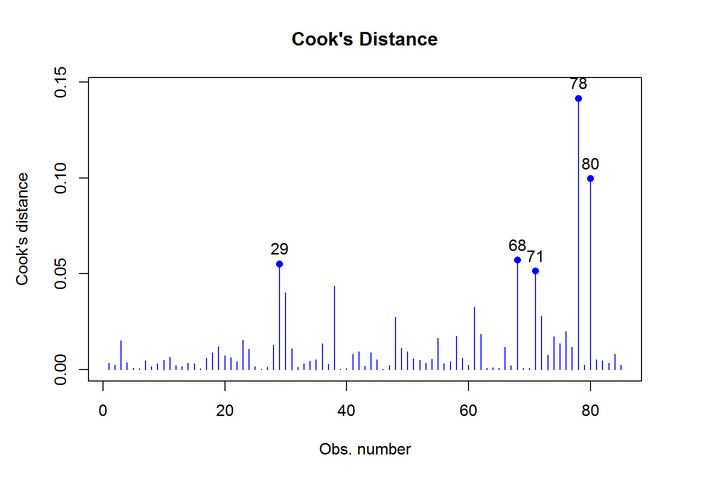
\includegraphics[width=0.9\linewidth]{images/CooksDistancePlot-JS-Roy}
\caption{}
\label{fig:CooksDistancePlot-JS-Roy}
\end{figure}
%For LME models, Cook's distance can be extended to model influence diagnostics by defining:
%\[ C_{\beta i} = {(\hat{\beta} - \hat{\beta}_{[i]})^{T}(\boldsymbol{X}^{\prime}\boldsymbol{V}^{-1}\boldsymbol{X}) (\hat{\beta} - \hat{\beta}_{[i]}) \over p}\]
%
%It is also desirable to measure the influence of the case deletions on the covariance matrix of $\hat{\beta}$.



\subsection{Local Influence}
\citet{cook86} gives a completely general method for assessing the influence of local departures from assumptions in statistical models, introducing methods for local influence assessment for classical linear models. These methods provide a powerful tool for examining perturbations in the assumption of a model, particularly the effects of local perturbations of parameters of observations. The local-influence approach to influence assessment is quite different from the case deletion approach, comparisons are of interest.

% % Beckman, Nachtsheim and Cook (1987)
\citet{Beckman} applied the \index{local influence}local influence method of Cook (1986) to the analysis of the LME model.  Other authors such as \citet{lesaffre1998local} have also extended these idea to LME models. 


While the concept of influence analysis is straightforward, implementation in LME models is more complex. Update formulae for fixed effects models are available only when the covariance parameters are assumed to be known. As such the local influence approach are not particularly useful in the context of method comparison, and so will not be considered further.






\subsection{Iterative and Non-Iterative Influence Analysis}




%----schabenberger page 8
For linear models, the implementation of influence analysis is straightforward, but for LME models the process is more complex. \citet{schabenberger} examines the use and implementation of
influence measures in LME models. \citet{schabenberger} highlights some of the issue regarding implementing LME model diagnostics, describing  the choice between \index{iterative influence analysis} iterative influence analysis and \index{non-iterative influence analysis} non-iterative influence analysis.
\citet{schabenberger} considers several important aspects of the use and implementation of influence measures in LME models, noting that it is not always possible to
derive influence statistics necessary for comparing full- and reduced-data parameter estimates. Closed-form expressions for computing the change in important model quantities might not be available.

\citet{schabenberger} describes the scenario wherein a data point is removed and the new estimate of the $G$ matrix is not positive definite. This may occur if a variance component
estimate now falls on the boundary of the parameter space \citep{schabenberger}. 

%%Non-Iterative
For classical linear models, it is not necessary to refit the model after removing a data point in order to measure the impact of an observation on the model. The change in fixed effect estimates, residuals, residual sums of squares, and the variance-covariance matrix of the fixed effects can be computed based on the fit to the full data alone, using update formulas \citep{sherman, hager1989}.


However, in LME models several important complications arise. Data points can affect not only the fixed effects but also the covariance parameter estimates on which the fixed-effects estimates depend. However update formulas are available only if one assumes that the covariance parameters are not affected by the removal of the observation in question. However, this is rarely a reasonable assumption.

For LME models, non-iterative methods are computationally efficient, but require the rather strong assumption that all covariance parameters are known, and thus are not updated, with the exception of the profiled residual variance.

Update formulas for ``\textit{leave-U-out}" estimates typically fail to account for changes in covariance parameters.  As the influence that each item would have on the variance estimate of a method comparison model is crucial, this substanitally negates their usefulness for Roy's Model.

Iterative influence diagnostics requiring fitting the model without the observations in question. Computation time is substantially longer, although this is balanced by algorithmic simplicity, with no assumptions beyond those used for the original model. A measure of total influence requires updates of all model parameters. This can only be achieved in general is by omitting observations or cases, then refitting the model. 


An iterative analysis may seem computationally expensive. Computing iterative influence diagnostics for $n$ observations requires $n+1$ mixed models to be fitted iteratively.
The execution times for iterative procedures are longer relative to non-iterative procedures, but are not so long that they would dissuade an analyst from using them.
Despite the addition execution time of iteratives
approaches, they are preferable for method comparison problems, as they can facilitate several complementary analyses concurrently. 


Iterative methods retain the potential for useful analyses, if applied at different stage of the modelling process. Diagnostic measures, specifically the DFBETA, have characteristics that would make them very useful at the exploratory stage of the method comparison process. Implicitly various assumptions about variance are used, but simultaneously an approach based on DFBETA can be used to assess if these assumptions are valid.




\subsection{Likelihood Distance}
In LME models fit by
\index{maximum likelihood} maximum likelihood (ML) or \index{restricted maximum likelihood} restricted maximum likelihood (REML), an overall influence measure is the \index{likelihood distance} likelihood distance \citep{CookWeisberg}.

\citet{west} examines a group of methods that examine various aspects of influence diagnostics for LME models. For overall influence, the most common approaches are the \textit{likelihood distance} and the \textit{restricted likelihood distance}.
The \index{likelihood distance} likelihood distance is a global summary measure that expresses the joint influence of the subsets of observations, $U$, on all parameters that were subject to updating. \citet{schabenberger} points out that the likelihood distance $LD(\psi_{(U)})$ is not the log-likelihood obtained by fitting the model to the reduced data set. Instead it is obtained by evaluating the likelihood function based on the full data set (containing all $n$ observations) at the reduced-data estimates.




%==========================================================%
%\subsubsection{Likelihood Distances}

The
procedure requires the calculation of the full data estimates
$\hat{\psi}$ and estimates based on the reduced data set
$\hat{\psi}_{(U)}$. The likelihood distance is given by
determining
\[
LD_{(U)} = 2\{l(\hat{\psi}) - l( \hat{\psi}_{(U)}) \}\]\[
RLD_{(U)} = 2\{l_{R}(\hat{\psi}) - l_{R}(\hat{\psi}_{(U)})\}
\]
Large values indicate that ${\hat{\theta}}$ and ${\hat{\theta}_\omega}$ differ considerably.



%For noniterative methods the following computational devices are used to compute (restricted) likelihood distances provided that the residual variance
%$\sigma^2$ is profiled.


\section{Model Diagnostics for Roy's Models}

Further to previous work, this section revisits case-deletion and residual diagnostics, and explores how approaches devised by  \citet{Galecki} can be used to appraise Roy's model. These authors specifically look at Cook's Distances and Likelihood Distances.
%	For the Roy Model, Cook's Distances may also be generated using the \textbf{\textit{predictmeans}}
%	





\begin{figure}[h!]
	\centering
	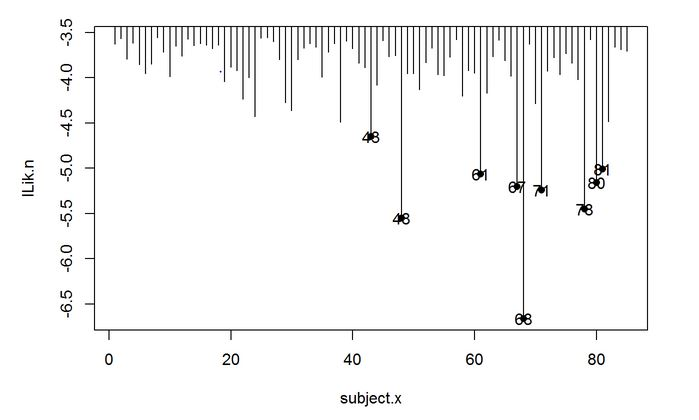
\includegraphics[width=0.7\linewidth]{images/LogLik-JS-Roy}
	\caption{}
	\label{fig:LogLik-JS-Roy}
\end{figure}





\citet{ARoy2009} establishes the equivalence of repeatability and within-item variability, and hence precision.  The method with the smaller within-item variability can be deemed to be the more precise.

A useful approach is to compute the confidence intervals for the ratio of within-item standard deviations, which is interpreted in the usual manner.
%

\citet[pb 93-95]{PB} give a description of how confidence intervals for the variance components are computed. Furthermore a complete set of confidence intervals can be computed to complement the variance component estimates. What is required is the computation of the variance ratios of within-item and between-item standard deviations.

A naive approach would be to compute the variance ratios by relevant F distribution quantiles. However, the question arises as to the appropriate degrees of freedom. Bootstrap methods for computing confidence intervals may be considered.

Further to previous work, this section revisits case-deletion and residual diagnostics, and explores how approaches devised by \citet{Galecki} can be used to appraise Roy's model. These authors specifically look at Cook's Distances and Likelihood Distances.
%For the Roy Model, Cook's Distances may also be generated using the \textbf{\textit{predictmeans}}
%




Applying the core principals of this methods to method comparison problem, case deletion diagnostics are used on the variance components of the Roy's model, specifically the ratio of between-subject variances and the within-subject covariances respectively.
\[ \mbox{BSVR} = \frac{\sigma^2_1}{\sigma^2_2} \phantom{makespace}  \mbox{WSVR} = \frac{d^2_1}{d^2_2} \]
These variance ratios are re-computed for each case removed, and may be analysed seperately or jointly for outliers, using standard techniques, such as the Grubbs tests.


The WSVR values are plotted against the corresponding BSVR values, with commonly used bivariate methods may be applied jointly to the both sets of data sets, e.g Mahalanobis distances. Confidence ellipses can be superimposed over the plot with minimal effort. Two ellipses are generated by this technique, a 50\% and 97.5\% confidence ellipse respectively. Outlying cases are idenified by the plot. Subject 68 is the most prominent case.

The subjects were ranked by Mahalanobis distance, with the top 10 being presented in the following table. Both sets of ratio are addtionally expressed as a ratio of the full model variance ratios.
\begin{center}
\begin{tabular}{|c|c|c|c|c|c|}
\hline
Subject (u) &  MD & WSVR$_{(u)}$ & WSVR (\%) & BSVR$_{(u)}$   & BSVR (\%)     \\ \hline \hline
68 & 44.7284   & 1.3615  & 0.9132   & 1.0353  & 0.9849 \\ \hline
30 & 16.7228   & 1.5045  & 1.0092   & 1.1024  & 1.0487 \\ \hline
71 & 11.5887   & 1.5210  & 1.0202   & 1.0932  & 1.0400 \\ \hline
80 & 11.0326   & 1.4796  & 0.9925   & 1.0114  & 0.9621 \\ \hline
38 & 10.3671   & 1.5011  & 1.0069   & 1.0917  & 1.0385 \\ \hline
67 & 10.1940   & 1.4308  & 0.9598   & 1.0514  & 1.0002 \\ \hline
43  & 7.6932   & 1.4385  & 0.9649   & 1.0511  & 0.9999 \\ \hline
72  & 4.7350   & 1.4900  & 0.9995   & 1.0262  & 0.9762 \\ \hline
48  & 4.4321   & 1.4950  & 1.0028   & 1.0280  & 0.9779 \\ \hline
29  & 4.3005   & 1.4910  & 1.0001   & 1.0769  & 1.0244 \\ \hline
\end{tabular}
\end{center}
From this table one may conclude that subjects 72, 48 and 29 are not particularly influential. Interestingly Subject 78, which was noticeable in the case deletion diagnostics for fixed effects, does not feature in this table.

\begin{figure}[h!]
\centering
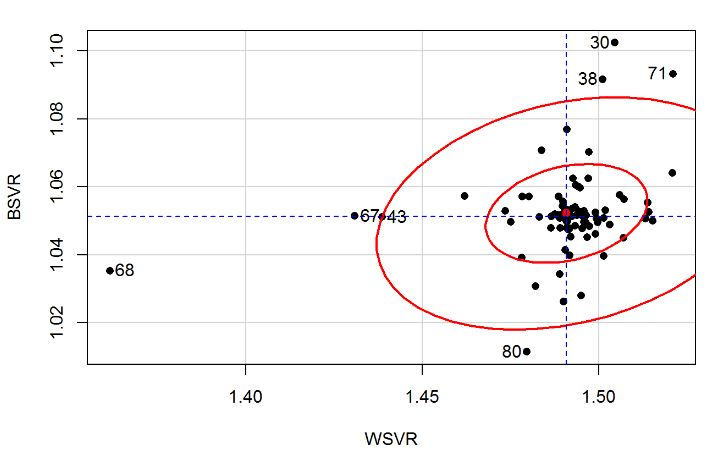
\includegraphics[width=0.9\linewidth]{08-plot1}
\caption{Identification of Prominent Observations}
\label{fig:08-plot1}
\end{figure}








\section{Agreement Criteria for Replicate Measurements}


Varying degrees of importances should be attached to each the three agreement criteria listed by \citet{Barnhart}. Between-item variance $d^2_i$ is fundamentally a measure of the variability of the item-wise means, as measured by method $i$, but it does contain limited information on the precision of that method. 

For conventional method comparison problems, both methods measures the same set of items using the same unit of measurement. Convergence to equality of between-item variance is inevitable as the number of items $n$ increases. Significantly different estimates for $d^2_1$ and $d^2_2$ should not be expected for any practical problem. 

Therefore a violation of third criterium (i.e. different between-item variances) criterium is contingent upon, and a  
possible consequence of, the violation of the other two agreement criteria. However, a violation of the third criterium will not occur in isolation. As noted elsewhere, the matter of inter-method bias can be easily accounted for, once detected. Both between-items and within-items variances must be calculated such that sources of variances are properly assigned, and to compute limits of agreement. However, testing the within-item criterium is the most informative analysis and therefore requires the most attention. 







\section{Using DFBETAs from LME Models to Assess Agreement}

 DFBETA and DFFITS are well known measures of influence. Emphasis shall be placed on DFBETA, but a brief discussion of DFFITS is merited as it potentially provides for useful techniques in method comparison. \citet{schabenberger} provides a mathematical desciption of both.


DFBETAS is a standardized measure of the absolute difference between the estimate with a particular
case included and the estimate without that particular case,, thus measuring the impact each observation has on a particular predictor \citep{belsley2005}. For LME models, the DFBETA is a measure that standardizes the absolute difference in parameter estimates between an LME model based on a full set of data, and a model from reduced data.

In general, large values of DFBETAS indicate observations that are influential in estimating a given parameter. There is no agreement as to the critical threshold for DFBETAs. \citet{belsley2005} recommend 2 as a general cutoff value to indicate influential observations and as a size-adjusted cutoff.  The cut-off value for DFBETAs is $\frac{2}{\sqrt{n}}$, where $n$ is the number of observations. 



\subsubsection{Using DFBETAs for Method Comparison}
For LME models, a value for DFBETAS is calculated for each of the $p$ fixed effects, and for each of the $n$ item. When the LME model is specified without an intercept term, as in Roy's Model, there is a set of DFBETAs corresponding to each measurement method, hence an $n \times p$ matrix.
% Correctly there will be $p+1$ DFBETAs (the intercept, $\beta_0$, and one $\beta$ for each covariate)

The LME approach proposed by \citet{ARoy2009} is constrained by computational tractability. Consequently a simpler LME formulation is used, one similar to that of \citet{BXC2008}. However one constraint that can be dispensed with is the restriction to two methods of measurement: we can now use any number of methods. The benefit of using this model is that metrics such as Cook's Distance and DFBETAs can be computed also.

For a method comparison study, DFBETAs can be used as a proxy measurement, allowing simple techniques to be used for assessing agreement. Suppose an LME model was formulated to model agreement for two or more methods of measurement, specifically with replicate measurements.

Hence, commonly used bivariate analyses constructed to compare each pair of methods, based on their respective sets of DFBETAs. Furthermore 95\% confidence ellipse can be constructed around these scatterplots. If the methods are to be agreement, the DFBETAs for each case would be the same for both methods. As such, agreement between any two methods can be visually inspected from a scatterplot of the DFBetas. 


%%
%%Furthermore, these measures form the basis of the analysis, rather than the estimates derived from the model. In the context of method comparison, these variables are the methods of measurement. Agreement will considered in the context of inter-method bias and the within-item variance ratio. Between-item variance ratio is not considered for this analysis.

Following the idea proposed by \citet{BA86}, an identity plot to visually inspect this relationship between sets of DFBETAs. Modern statistical software usually allows for the creation of co-plots, so a grid of identity plots may be easily rendered for comparing each pair of methods.

If the lack of agreement is caused, in part or in full, by differing within-item variances, there would be differing DFBETAs for each pair of methods. If the points align along the line of equality, then both methods can be said to be in agreement for within item variance. However DFBETAs are not useful for determining inter-method bias. 

If there is good agreement between methods, or if lack of agreement is caused by inter-method bias only, the DFBETA values will be almost identical for each subject. Therefore this plot should be used in conjunction with a Bland-Altman plot. If lack of agreement is indicated, a comprehensive analysis using Roy's framework can be used to formally test for various causes of lack of agreement \citep{ARoy2009}.



For an LME model fitted to the Systolic Blood Pressure data, the results tabulated below can be produced.  Cases can be ranked by the Cook's Distance, with the top 6 being presented below). The remaining columns are the DFBeta for each of the fixed effects, for each of the 85 subject.
\begin{center}
\begin{tabular}{|c|c|c|c|c|} \hline
Subject &    Cook's D  &    Method J  &   Method R  & Method S \\ \hline \hline
78 & 0.6155 & -0.0293 & -0.0338 & 0.2954  \\ \hline
80 & 0.4159 & -0.0630 & -0.0651 & 0.2123  \\ \hline
68 & 0.2253 & -0.0533 & -0.0506 & 0.1555  \\ \hline
72 & 0.0934  & 0.0238  & 0.0241 & 0.1617  \\ \hline
48 & 0.0870  & 0.0214  & 0.0314 & 0.1581  \\ \hline
30 & 0.0711  & 0.2692  & 0.2621 & 0.1581  \\ \hline
\end{tabular}
\end{center}
For DFBETA identity plots are presented in Figure~\ref{fig:04-DFbetaplots}. This set of plots indicate agreement between methods J and R in terms of within-item variance, while severe lack of agreement exists between these methods and the third method S, as is the conclusion of \citet{ARoy2009}.
\begin{figure}[h!]
\centering
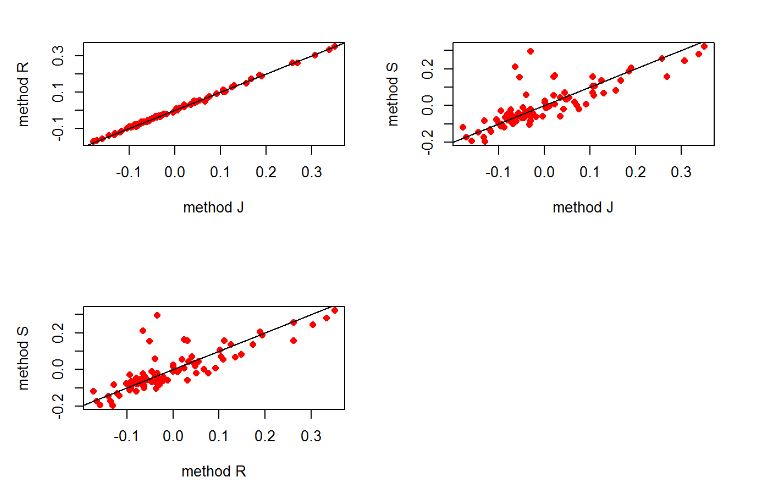
\includegraphics[width=1.1\linewidth]{images/04-DFbetaplots}
% \caption{}
\label{fig:04-DFbetaplots}
\end{figure}



%Other analyses may be used to complement these plots. The Pearson Correlation coefficient of the DFBETAs can be used in conjection with this analysis. A high correlation confirms good agreement, thouhg no threshold value for agreement is suggested.

The Bonferroni Outlier Test and Cook's Distance values can be used to identify unusual cases, when the relationship between sets of DFBETA is modelled as a (classical) linear model. In this model, the covariates should be homoskedastic. A test for non-constant variance may be used to verify this. 


As an alternative to scatterplots, a mean difference plot could be used to assess agreement of with-item variance. This mean-difference plot differs from the Bland-Altman plot in that the plot is denominated in terms of DFBETA values, and not in measurement units. Here two of the three pairs of methods are compared on the same plot, red points indicate the J-R comparison while blue points are for the J-S comparison.

\begin{figure}[h!
]
\centering
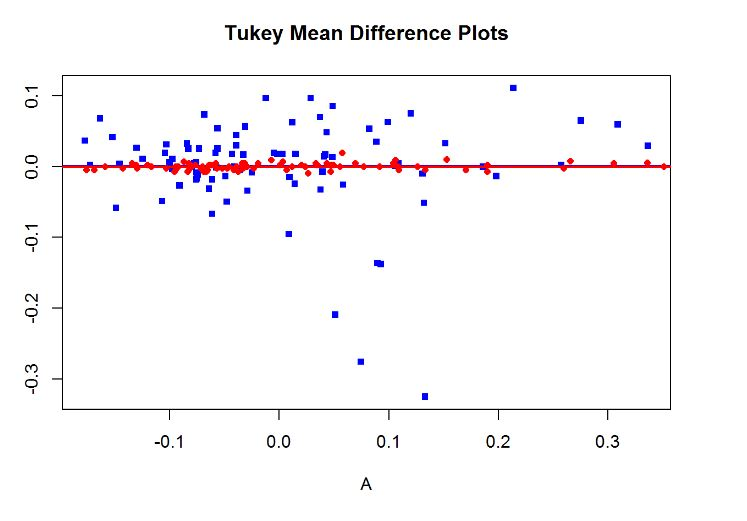
\includegraphics[width=0.7\linewidth]{images/04-TMDplot}

\end{figure}







\bibliography{2017bib}



\end{document}


%---------------------------------------------------------------------------------------------------%


